%!TEX root = ../per_st_tk.tex

%\begin{frame}{A more abstract viewpoint}
%	\pause
%	Operads control algebraic structures.
%
%	\bigskip\pause
%	The operad $\cC om$ controls cocommutative and coassociative coalgebras.
%
%	\bigskip\pause
%	An $E_\infty$-operad is an $\sym$-cofibrant resolution of $\cC om$.
%
%	\bigskip\pause
%	Controls coalgebras cocomm. and coassoc. up to coherent homotopies.
%
%	\bigskip\pause
%	$E_\infty$-structures have a long history:
%	\smallskip\pause
%	\begin{itemize}
%		\item (co)homology operations,
%		\item recognition of infinite loop spaces,
%		\item algebraic models of the homotopy category.
%	\end{itemize}
%
%	\bigskip\pause
%	\colorit{Fact}:
%	Fully deriving its diagonal map, the chains of a space form an $E_\infty$-coalgebra.
%
%	\bigskip\pause
%	\colorit{Principle} (Quillen, Sullivan, Mandell, ...): \\
%	\textbf{All} homotopy information of spaces is in this algebraic model.
%
%	\bigskip\pause
%	\colorit{Question}: How explicit can this $E_\infty$-structure be made?
%\end{frame}
%
%\begin{frame}{Explicit $E_\infty$-structure on (co)chains}
%	\pause
%	\colorit{Theorem (Med.)} \\
%	The collection of maps $\gchains(\gsimplex^n) \to \gchains(\gsimplex^n)^{\otimes r}$ obtained from compositions of
%	\begin{align*}
%		\Delta &\colon \gchains(\gsimplex^n) \to \gchains(\gsimplex^n)^{\otimes 2}
%		\qquad \text{(AW diagonal)} \\
%		\ast &\colon \gchains(\gsimplex^n)^{\otimes 2} \to \gchains(\gsimplex^n)
%		\qquad \text{(Join map)}
%	\end{align*}
%	defines an $E_\infty$-coalgebra on simplicial chains.
%
%	\bigskip\pause
%	\colorit{Join map} \\
%	\qquad\qquad \scalebox{0.7}{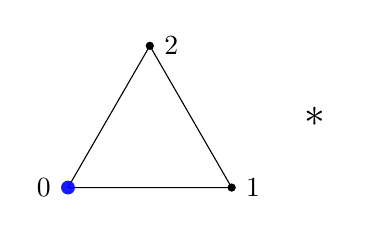
\begin{tikzpicture}[scale=.6]
\coordinate (A) at (210:2);
\coordinate (B) at (-30:2);
\coordinate (C) at (90:2);

\draw[draw=black] (A) -- (B) -- (C) -- (A);

\node[circle,fill=blue, opacity=.9, inner sep=0pt,minimum size=5pt, label=left:{0}] (a) at (A) {};
\node[circle,fill=black,inner sep=0pt,minimum size=3pt, label=right:{$1$}] (a) at (B) {};
\node[circle,fill=black,inner sep=0pt,minimum size=3pt, label=right:{$2$}] (a) at (C) {};

\node[scale=1.5] at (3.5,0.5) {$\ast$};
\end{tikzpicture}
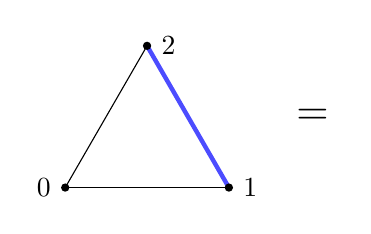
\begin{tikzpicture}[scale=.6]
\coordinate (A) at (210:2);
\coordinate (B) at (-30:2);
\coordinate (C) at (90:2);

\draw[draw=blue,  ultra thick, draw opacity=.7] (B) -- (C);
\draw[draw=black] (C) -- (A);
\draw[draw=black] (A) -- (B);

\node[circle,fill=black,inner sep=0pt,minimum size=3pt, label=left:{$0$}] (a) at (A) {};
\node[circle,fill=black,inner sep=0pt,minimum size=3pt, label=right:{$1$}] (a) at (B) {};
\node[circle,fill=black,inner sep=0pt,minimum size=3pt, label=right:{$2$}] (a) at (C) {};

\node[scale=1.5] at (3.5,.5) {=};
\end{tikzpicture}
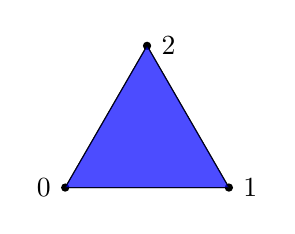
\begin{tikzpicture}[scale=.6]
\coordinate (A) at (210:2);
\coordinate (B) at (-30:2);
\coordinate (C) at (90:2);

\draw[draw=black] (A) -- (B) -- (C) -- (A);

\node[circle,fill=black,inner sep=0pt,minimum size=3pt, label=left:{$0$}] (a) at (A) {};
\node[circle,fill=black,inner sep=0pt,minimum size=3pt, label=right:{$1$}] (a) at (B) {};
\node[circle,fill=black,inner sep=0pt,minimum size=3pt, label=right:{$2$}] (a) at (C) {};

\draw[draw, fill=blue, opacity=.7] (A) -- (B) -- (C) -- (A);
\end{tikzpicture}}
%
%	\bigskip\pause
%	\colorit{Other versions} \\
%	\colorit{1)} Cubical (Kaufmann--Med.) \\
%	\colorit{2)} Multisimplicial (Med.--Pizzi--Salvatore).
%\end{frame}
